\subsection*{Wi-Fi Data Link Layer}

The next layer in the OSI model is the Data Link Layer.
The Data Link Layer consists of Medium Access - and Logic Link Control functionalities.


According to \textcite{kauffels_wireless_2002}, the medium access control functionalities cover network entry - ,network authentication - and media access methods.
The author explains, that every \ac{AP} send beacon frames periodically to synchronise its stations in the \ac{BSS} and that the beacon frame contains the \ac{SSID}, which identifies the \ac{BSS} or \ac{ESS} of the station. \textcite{sauter_wireless_2022} adds that a beacon frame contains a \SI{16}{\bit} - long capability information element. Each bit here signals that the \ac{AP} provides a particular function or has a specific feature.

\textcite{kauffels_wireless_2002} explains the procedure for network entry of a station. A station can use the passive or the active scanning mode. In passive scanning mode, the station listens for a beacon frame in the various transmission channels. Alternatively, in active scanning mode, a station can also send out a probe frame. This can contain an already known \ac{SSID} to test the presence of the \ac{AP}. To get an \ac{AP} in range, the probe-frame can also contain a broadcast SSID that causes all nearby \ac{AP}s to respond. The response of an \ac{AP} to the probe frame is the probe-response frame, which contains the same information as a beacon frame. With the information from the beacon frame, a station can start the authentication process.

For this process, \textcite{kauffels_wireless_2002} names the two methods Open System Authentication and Shared Key Authentication. \textcite{sauter_wireless_2022} explains that Open System Authentication is based on a device making an authentication request to the \ac{AP}. If the \ac{AP} answers with a positive status in the Authentication Frame, the station is included in the \ac{BSS}. The actual encryption and authentication is then performed by the \ac{WPA} functions. The author points out that Shared Key Authentication is no longer used today.

 the IEEE 802.11 standard describes the two media access methods \ac{DCF} and \ac{PCF}.

\textcite{sauter_wireless_2022} explains that \ac{DCF} is based on the media access method \ac{CSMACA}. In \ac{CSMACA} a device that is willing to transmit senses in the air transmission medium for a transmitting activity. If no other device is transmitting, the device can transmit. In the case of transmit activity, the terminal must wait at least until the transmission and \ac{DIFS} are over.
Since data transmission via the air transmission medium is very vulnerable to errors, the standard IEEE 802.11 requires that each received packet must be confirmed with an \ac{ACK} frame.
The \ac{DIFS} ensures that an \ac{ACK} frame can be sent before another station uses the same channel to send a data frame.
To avoid multiple devices transmitting at the same time after \ac{DIFS}, each ready-to-transmit device determines a random backoff time. The device with the shortest backoff time transmits next and all other ready-to-transmit devices restart the media access procedure. In case two devices start sending next because they both randomly chose the shortest backoff time, the transmitted signal will interfere and the packets will not be answered with an \ac{ACK} frame.
In case of such a faulty transmission, the backoff time of the ready-to-transmit devices can increase exponentially afterwards.

To share the knowledge of a transmission time and the subsequently interframe space, a packet contains a \ac{NAV} that specifies the time the air transmission medium is used.

In various network architectures the "hidden station"-problem may occur. As you can see in \autoref{fig:hidden_station}, Station A is not able to sense a transmission of station B and vise versa. In case of simultaneous transmission of both stations, interference around the \ac{AP} may occur.
\begin{figure}%
	\centering
	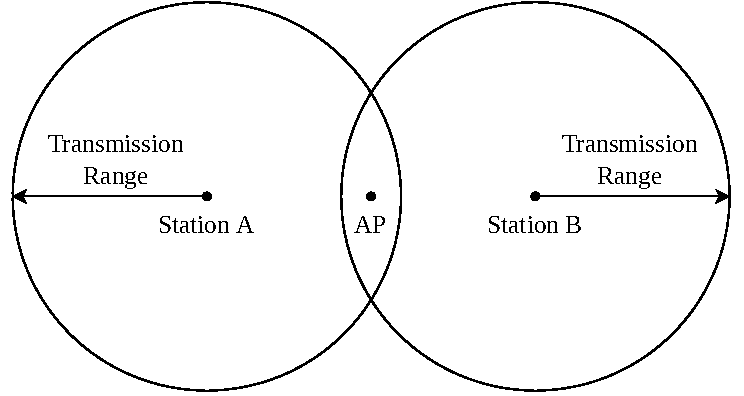
\includegraphics[width=0.75\textwidth]{figures/hidden_station.pdf}
	\caption{Hidden Station Problem}%
	\label{fig:hidden_station}%
\end{figure}


Um das hidden station problem zu umgehen kann eine Station nach \textcite{sauter_wireless_2022}
Point coordinator
ohne Wettbewerb mit optionaler Priorisierung

PIFS interval kürzer,
beacon frame
CF Parameter set-element
\todo{nicht genauer eingehen, weil nicht relevant für die Arbeit? Darf ich das schreiben?}

CSMA /CA
Point Coordination Function

\textcite{sauter_wireless_2022}
DCF oberbegriff für CSMA /CA


Short Interframe Space SIFS ACK Frame

Hidden Station Problem
CTS and RTS

IEEE 802.11e DCF erweiterung für Video Streaming

CSMA CA Backoff zeit
Network allocation Vector NAV Zeitspanne Datensendungsdauer

MAC Header

Netzeintritt:
passives und Aktives Scanning
Service Set Identifier
Timing Synchronisationsfunktion TSF Timer-Wert

\textcite{sauter_wireless_2022}
every package management or usage data send ackknowledgement

Hidden Station Szenario
Reservieren
RTS CTS
meist nicht konfiguriert / ausgeschalten, bei großen Paketen sinnvoll



Authentifizierung
- Open System -Authentification
- Shared key Authentification
(nach neu nicht mehr verwendet